\chapter{Grundlagen}
\label{Grundlagen}

Für den praktischen Teil dieser Arbeit in Abschnitt \ref{praktischer Teil} werden mit Hilfe von CGP unterschiedliche Testprobleme gelöst. 
Für das Verständnis dieses Teil werden einige Grundkenntnisse vorausgesetzt, welche in diesem Abschnitt näher betrachtet werden.\newline
CGP ist eine Art von GP, welches verwendet wird, um unterschiedliche Probleme zu lösen.
Dabei wird der Maschine allerdings nicht beigebracht, wie diese Probleme zu lösen sind.
Stattdessen lernt sie eigenständig über mehrere Iterationen hinweg das Ausgangsproblem zu lösen.
Dies geschieht angelehnt an die Darwin’sche Theorie der biologischen Evolution. \cite{milad_taleby_ahvanooey_survey_2019} \newline
Um den grundlegenden Aufbau von CGP zu erläutern, wird die folgende Abbildung \ref{fig:aufbauCGP} verwendet:

\begin{figure}[H]
    \centering
    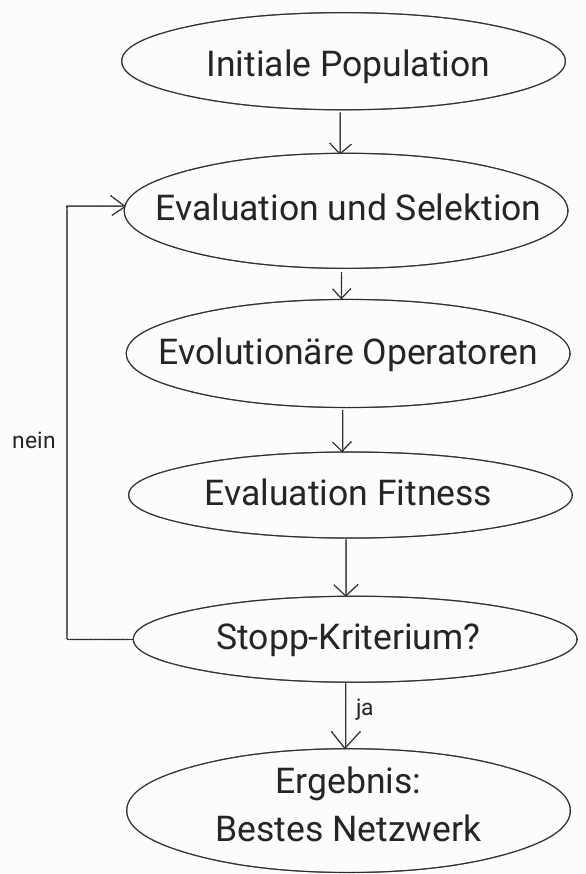
\includegraphics[scale = 0.43]{Bilder/AufbauCGPVorgehenNachbildung.png}
    \caption{Aufbau CGP, angelehnt an \cite{torabi_using_2022}}
    \label{fig:aufbauCGP}
\end{figure}

Die Abbildung \ref{fig:aufbauCGP} zeigt den grundlegenden Ablauf innerhalb von CGP.
Dabei lernt das System über mehrere Iterationen hinweg die beste Lösung eines Problems.
Die folgenden Unterkapitel beziehen sich jeweils auf einen Knoten des Graphen und erläutern diesen genauer.


\section{Aufbau CGP und initiale Population}
\label{sec:initialePopulation}
Dieser Abschnitt bezieht sich auf die Paper \cite{miller_cartesian_2020}, \cite{torabi_using_2022} und \cite{milad_taleby_ahvanooey_survey_2019}.
Außerdem werden Erkenntnisse aus dem Quellcode von Cui verwendet \cite{cuihen_cuihencgp_with_crossover_strategies_2024}.\\
Die \emph{Population} von CGP ist eine Menge von \emph{Chromosomen}, auch Individuen genannt.
Chromosome sind individuelle Möglichkeiten ein komplexes Ausgangsproblem zu lösen.
Jedes Chromosom ist in CGP ein gerichteter, azyklischer Graph, bestehend aus \emph{Eingangsknoten}, \emph{Rechenknoten} und \emph{Ausgangsknoten}.
Dabei gibt es zwei Darstellungsmöglichkeiten für ein Chromosom. 
Anhand der folgenden Abbildung \ref{fig:genoPhänoGesamt} kann beispielhaft dargestellt werden, wie die Chromosome in CGP aufgebaut sind und funktionieren.

\begin{figure}[H]
	\centering
	\begin{subfigure}[b]{\textwidth}
		\centering
		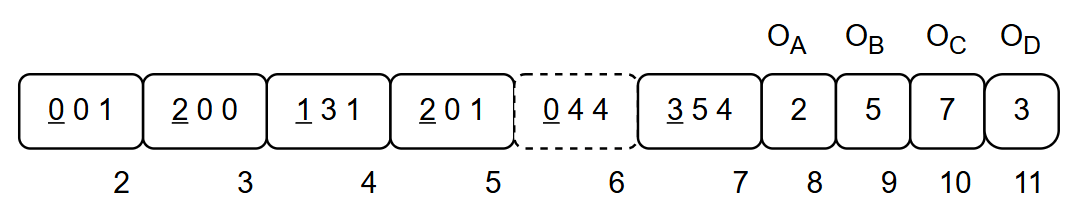
\includegraphics[scale = 0.45]{Bilder/TorabiBeispielGenotypNeu.png}
		\caption{Beispiel Genotyp}
		\label{fig:genotypNeu}
	\end{subfigure}
	
	\hfill
    
    \begin{subfigure}[b]{\textwidth}
    	\centering
    	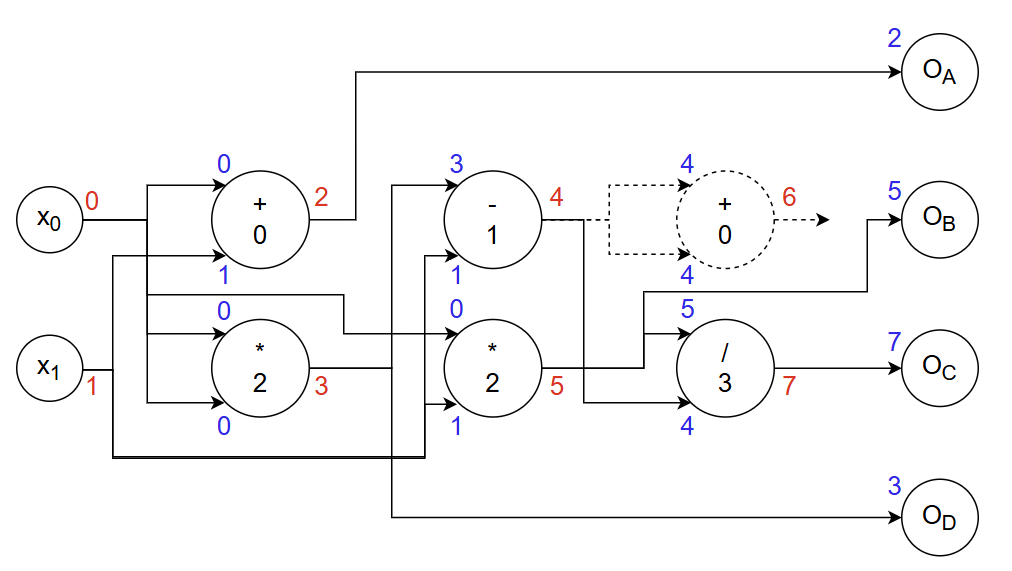
\includegraphics[scale = 0.45]{Bilder/BeispielChromosom.png}
    	\caption{Beispiel Phänotyp}
    	\label{fig:phänotyp}
    \end{subfigure}
    \caption{Darstellungsmöglichkeiten eines Chromosoms, angelehnt an \cite{torabi_using_2022}}
    \label{fig:genoPhänoGesamt}
\end{figure}


Anhand Abbildung \ref{fig:phänotyp} lässt sich die klassische Struktur von CGP erkennen:
Es handelt sich um einen gerichteten, azyklischen Graphen mit Ein- und Ausgängen.
In diesem Beispiel werden die beiden Systemeingänge $x_0$ und $x_1$ vorausgesetzt, welche durch Eingangsknoten zur Verfügung gestellt werden.
Aus diesen Eingaben sollen anschließend durch verschiedene Berechnungen die Ausgänge resultieren.
In diesem Fall werden vier Systemausgänge berechnet, die durch die Ausgangsknoten $O_A$ – $O_D$ dargestellt werden.
Zwischen den Ein- und Ausgangsknoten liegen die Rechenknoten.
Diese werden verwendet, um verschiedene Rechenoperationen an den Eingangsknoten auszuführen, bis schließlich die Inhalte der Ausgangsknoten als Ergebnis resultieren.
Die Rechenoperationen, die von den Rechenknoten ausgeführt werden, werden je nach Anwendungsfall definiert und codiert.
In diesem Beispiel ergibt sich folgende Kodierung:

\begin{table}[H]
    \centering
    \begin{tabular}{c | c}
       \textbf{Rechenoperation} & \textbf{Kodierung} \\ \hline
        + & 0 \\ \hline
        - & 1 \\ \hline
        * & 2 \\ \hline
        / & 3
    \end{tabular}
    \caption{Kodierung der Rechenoperationen}
    \label{table:kodierung}
\end{table}

Diese Kodierungen werden in Abbildung \ref{fig:phänotyp} innerhalb der Knoten angegeben und stellen die erste (unterstrichene) Zahl innerhalb des Arrays in Abbildung \ref{fig:genotypNeu} dar.
Die umrandeten Teile des gesamten Arrays stellen jeweils einen Knoten des Graphen dar und werden folgend Array-Blöcke genannt.
Unterhalb dieser Array-Blöcke wird jeweils der Index des zugehörigen Knotens angegeben.
Im CGP-Graph wird dieser Index am Ausgang des jeweiligen Knotens (rot) angezeigt.\newline
Des Weiteren werden in Abbildung \ref{fig:genotypNeu} die Eingangskanten für jeden Knoten angegeben. 
In diesem Beispiel hat jeder Rechenknoten zwei Eingänge und jeder Ausgangsknoten hat jeweils nur einen Eingang, in dem das Ergebnis eines Rechenknoten weitergeleitet und ausgegeben wird.
Die Knoteneingänge sind in Abbildung \ref{fig:phänotyp} blau markiert.
Hier werden die Indices derjenigen Knoten angegeben, deren Ausgangswerte verwendet werden.
Diese spiegeln sich ebenfalls in Abbildung \ref{fig:genotypNeu} wider: hier werden die Knoteneingänge innerhalb der Array-Blöcke als nicht-unterstrichene Indices angegeben.
Damit ergibt sich eine vollständige Beschreibung eines Knotens, indem einem Index Eingänge und gegebenenfalls eine Rechenoperation zugeschrieben werden.\newline
Durch dieses Beispiel wird ebenfalls ersichtlich, was die Eingangsknoten eines Chromosoms ausmacht:
Sie geben die Systemeingänge wieder, ohne diese auf irgendeine Weise zu verarbeiten.
Aus diesem Grund müssen die Eingangsknoten nicht im Genotyp aufgezeigt werden, um sie vollständig zu beschreiben, denn sie weisen weder Eingänge noch Rechenoperationen auf, die beschrieben werden müssten.

Die beiden Darstellungsmöglichkeiten eines Chromosoms werden wie in Abbildung \ref{fig:genoPhänoGesamt} \emph{Genotyp} und \emph{Phänotyp} genannt.
Der Phänotyp resultiert dabei aus dem Genotyp.
Der Genotyp ist das volle Individuum, während der Phänotyp die Dekodierung dessen ist.
Die Lösung des CGPs ist dementsprechend ein Phänotyp, also die Dekodierung des besten Individuums des CGPs.
Der Genotyp- und Phänotyp-Raum können sich dabei stark voneinander unterscheiden. \cite{eiben_introduction_2015}
Dies lässt sich dadurch erklären, dass nicht alle Teile des Genotyps für die Berechnung des Endergebnisses verwendet werden.
Diejenigen Anteile, die für die Berechnung der Lösung nicht gebraucht werden, werden \emph{inaktive Knoten} genannt.
So ein inaktiver Knoten wird in Abbildung \ref{fig:genotypNeu} durch gestrichelte Linien dargestellt.
Da der Phänotyp die Lösung des CGPs ist, müssen inaktive Knoten auch nicht im Phänotyp dargestellt werden, denn diese finden für die Berechnung keine Verwendung.
Der Vollständigkeit halber wird der inaktive Knoten aus Abbildung \ref{fig:genotypNeu} auch in Abbildung \ref{fig:phänotyp} aufgenommen.
So können also verschiedene Genotypen zum gleichen Phänotyp führen, indem sich verschiedene Genotypen nur anhand ihrer inaktiven Knoten unterscheiden.
Da der Phänotyp auch den auszuführenden Programmcode darstellt, können auch verschiedene Genotypen zum gleichen Ergebnis führen.
Dies kann die Weiterentwicklung der Chromosomen stören, indem beispielsweise nur inaktive Knoten eines Chromosoms angepasst werden.
Das kann sich wiederum negativ auf die Trainingsdauer auswirken.
Eine nähere Erklärung wird in Abschnitt \ref{subsec:Mutation} gegeben.\\
Ob ein Knoten für die Berechnung der Lösung verwendet wird oder nicht, hängt davon ab, ob ein nachfolgender Knoten auf dessen Ausgang zugreift.
Um aktive Knoten von inaktiven Knoten zu unterscheiden, werden demnach zuerst die Ausgangsknoten betrachtet, die offensichtlich für die Auswertung der Ausgabe verwendet werden.
Anschließend werden iterativ die Eingangskanten der Rechenknoten zurückverfolgt, bis man schließlich bei den Eingangsknoten des Graphen ankommt.

Schließlich soll anhand der eingeführten Abbildungen \ref{fig:genotypNeu} und \ref{fig:phänotyp} ein Beispiel berechnet werden:\newline
Angenommen werden die Systemeingänge $x_0$ = 10 und $x_1$ = 20.
Demnach sind die Ausgänge der beiden Eingangsknoten mit den Indices 0 und 1 gleich den Werten 10 und 20.
Der erste Rechenknoten (Index = 2) verwendet die beiden Eingangsknoten (Indices = 0 und 1) als Eingänge und besitzt die Rechenfunktion +.
Demnach ist das Ergebnis des Rechenknotens 10 + 20 = 30.
Führt man dieses Vorgehen für die restlichen Rechenknoten aus, ergeben sich folgende Ergebnisse:

\begin{table}[H]
    \centering
    \begin{tabular}{c|c|c|c|c}
       \textbf{Knoten} & \textbf{Eingänge} & \textbf{Werte Eingänge} & \textbf{Rechenoperation} & \textbf{Ausgangswert} \\ \hline
        2 & 0; 1 & 10; 20 & 10 + 20 & 30 \\ \hline
        3 & 0; 0 & 10; 10 & 10 * 10 & 100 \\ \hline
        4 & 3; 1 & 100; 20 & 100 - 20 & 80 \\ \hline
        5 & 0; 1 & 10; 20 & 10 * 20 & 200 \\ \hline
        7 & 5; 4 & 200; 80 & 200 / 80 & 2,5
    \end{tabular}
    \caption{Ergebnisse Rechenknoten}
    \label{table:ergebnisseRechenknoten}
\end{table}

Die Ausgangsknoten geben die jeweiligen Ergebnisse der Eingangs- oder Rechenknoten zurück.
In diesem Beispiel werden durch das Chromosom folgende Ausgänge aus den beiden Eingängen (10; 20) berechnet:

\begin{table}[H]
    \centering
    \begin{tabular}{c|c|c}
       \textbf{Ausgangsknoten} & \textbf{Index Eingang} & \textbf{Wert des Ausgangsknotens} \\ \hline
        $O_A$ & 2 & 30 \\ \hline
        $O_B$ & 5 & 200 \\ \hline
        $O_C$ & 7 & 2,5 \\ \hline
        $O_D$ & 3 & 100
    \end{tabular}
    \caption{Ergebnisse Ausgangsknoten}
    \label{table:ergebnisseAusgangsknoten}
\end{table}

Zusammengefasst hat das Beispielchromosom aus dem Eingangstupel (10; 20) das Ausgangstupel (30; 200; 2,5; 100) berechnet.\\

Wie bereits erläutert, ist die Population in CGP eine Menge an Chromosomen, also eine Menge an gerichteten, azyklischen Graphen, die aus definierten Systemeingaben Ausgaben berechnen können.
Diese Population wird zu Beginn zufällig initialisiert.
Dabei werden folgende Angaben vorausgesetzt:
\begin{itemize}
    \item Größe der Population
    \item Anzahl der Systemeingänge
    \item Anzahl der Systemausgänge
    \item Anzahl der Rechenknoten pro Chromosom
\end{itemize}
Im Initialisierungsprozess werden für jedes Chromosom pro Knoten zufällige Eingangskanten und gegebenenfalls Rechenoperationen bestimmt.
Dabei muss beachtet werden, dass es sich anschließend um einen azyklischen Graphen handeln muss.

Nachdem die initiale Population erstellt wurde, erfolgt der erste \emph{Evaluations-} und \emph{Selektionsschritt}. 
Der folgende Abschnitt \ref{sec:evalUndSelektion} erläutert, wie diese Schritte ausgeführt werden.


\section{Evaluation und Selektion}
\label{sec:evalUndSelektion}

Der erste Selektionsschritt in CGP startet mit einer zufällig initialisierten Population, wie sie in Abschnitt \ref{sec:initialePopulation} beschrieben wird.
In dieser initialen Population ist die Performance der einzelnen Individuen rein zufällig.
Das Ziel von CGP ist es, die Performance über Generationen hinweg zu verbessern, bis schließlich eine (nahezu) perfekte Lösung eines Problems gefunden wird.
GP im Allgemeinen richtet sich nach dem darwin'schen Prinzip des Überlebens der Stärkeren.
Demnach werden die performantesten Chromosomen verwendet, um die nächste Generation der Population zu erzeugen. \cite{koza_survey_1995}

Um zu bestimmen, welche Individuen die beste Performance aufweisen, muss eine numerische Bewertung erfolgen.
Diese wird durch die \emph{Fitness} der einzelnen Chromosomen bestimmt. \cite{koza_survey_1995}
Wie der Fitnesswert berechnet wird, hängt von den zu lösenden Problemen ab.
Beispielsweise verwenden Cui et al. für symbolische Regressionsprobleme den mittleren absoluten Fehler zwischen korrekter Lösung und tatsächlicher Lösung für einen Evaluationsdatensatz. \cite{affenzeller_positional_2024}

Koza beschreibt in seinem Paper, dass für die Selektion der Eltern der nächsten Generation, jedem Chromosom ein Wahrscheinlichkeitswert zugewiesen wird.
Dieser hängt von dessen Fitness ab.
Anschließend wird eine definierte Anzahl an Eltern selektiert, wobei die Wahrscheinlichkeitswerte dafür sorgen, dass fittere Individuen die größere Chance haben, selektiert zu werden.
Selektion heißt dabei, dass das Chromosom unverändert in die nächste Generation kopiert wird. \cite{koza_survey_1995}\newline
Dies ist ein Weg dafür zu sorgen, dass das Prinzip nach Darwin eingehalten wird und somit die fitteren Chromosomen \glqq überleben\grqq. 
Eine andere Möglichkeit, dies zu erreichen, ist die Verwendung von sogenannten \emph{Elitisten}.
Die fittesten Individuen einer Generation werden dabei als Elitisten erwählt und werden für die darauf folgende Generation selektiert. \cite{krawiec_genetic_2013}
Für die Auswahl der Elitisten wird in dieser Arbeit der \emph{neutral search Algorithmus} verwendet.
Dieser wird relevant, falls innerhalb einer Generation ein Elter-Chromosom und ein Kind-Chromosom die gleiche Fitness aufweisen.
In diesem Fall wird stets das Kind-Chromosom als Elitist ausgewählt.
Dies führt dazu, dass anschließend bessere Nachkommen erzeugt werden können. \cite{mernik_refining_2022}\newline
Mit dem in dieser Arbeit verwendeten Selektionsverfahren namens \emph{($\mu$ + $\lambda$)-Evolution Strategy (ES)} wird dieser Ansatz verfolgt. 
Dabei werden jeweils $\mu$-viele Eltern für die folgende Generation selektiert.
Im Standard-CGP wird $\mu$ mit 1 belegt.
Die restlichen Individuen der Population ($\lambda$-viele) werden anschließend durch \emph{Mutation} aus dem Elter-Chromosom gebildet. \cite{da_silva_cartesian_2018}
Da für den \emph{Rekombinationsschritt} jeweils zwei Eltern-Chromosomen gekreuzt werden, muss für $\mu$ ein Wert größer als 1 gewählt werden, falls Rekombination ausgeführt wird.
Um eine bessere Vergleichbarkeit zu gewährleisten, werden im praktischen Teil auch unterschiedliche $\mu$-Werte gewählt, selbst wenn keine Rekombination ausgeführt wird.\newline
Die folgenden Abschnitte \ref{sec:evolutionäreOperatoren} und \ref{subsec:Mutation} erläutern die Funktionsweise von Rekombination und Mutation.


\section{Evolutionärer Operator: Rekombination}
\label{sec:evolutionäreOperatoren}
Nachdem die Selektion der Eltern-Chromosome erfolgt ist, wie in Abschnitt \ref{sec:evalUndSelektion} beschrieben, können im nächsten Schritt die evolutionären Operationen ausgeführt werden, die die Nachkommen aus den Eltern erzeugen. \\
Der erste evolutionäre Operator, der verwendet wird, ist die Rekombination.
Dabei werden jeweils zwei zufällig ausgewählte Eltern-Chromosomen kombiniert und somit zwei neue (Nachkommen-)Chromosomen erzeugt \cite{kalkreuth_comprehensive_2020}. 
Der Rekombinationsschritt wird so oft ausgeführt, bis die Population dieser Generation gefüllt ist.\\
Innerhalb dieser Arbeit werden unterschiedliche Rekombinationsalgorithmen für die Nachwuchserzeugung miteinander verglichen.
Diese werden in den folgenden Absätzen \ref{subsubsec:onePointCrossover} bis \ref{subsec:rekombinationsraten} näher erläutert.

\subsection{One-Point Rekombination}
\label{subsubsec:onePointCrossover}
Das erste Standard-Rekombinationsverfahren, das in dieser Arbeit verwendet wird, ist die \emph{One-Point Rekombination}.
Für die Grundlagen aus diesem Abschnitt wurde \cite{pavai_survey_2017} als Quelle verwendet.\\
Der One-Point Rekombinationsalgorithmus soll anhand folgender Beispielabbildung \ref{fig:onePointGesamt} erläutert werden:

\begin{figure}[H]
	\centering
	\begin{subfigure}[b]{\textwidth}
		\centering
		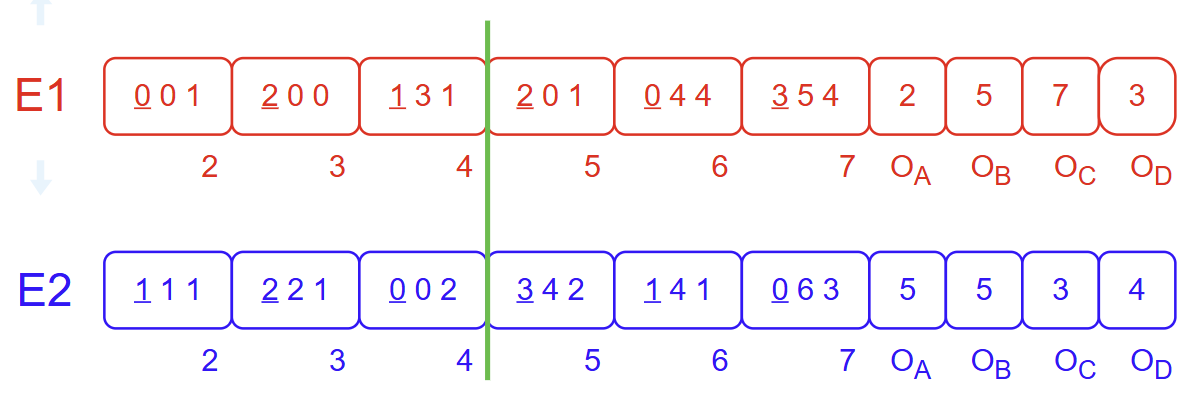
\includegraphics[scale = 0.77]{Bilder/BeispielOnePointCrossover.png}
		\caption{Eltern-Chromosomen One-Point Rekombination}
		\label{fig:onePointCrossoverEltern}
	\end{subfigure}
	
	\hfill
	
	\begin{subfigure}[b]{\textwidth}
		\centering
		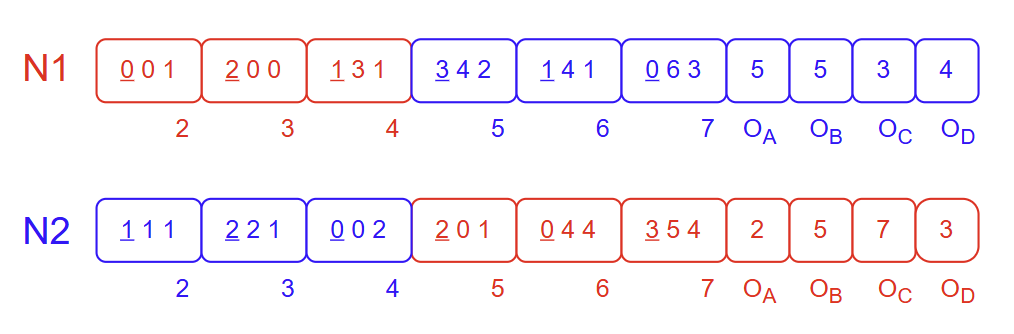
\includegraphics[scale = 0.55]{Bilder/BeispielOnePointCrossover2.png}
		\caption{Nachwuchs-Chromosomen One-Point Rekombination}
		\label{fig:onePointCrossoverNachwuchs}
	\end{subfigure}
	\caption{One-Point Rekombination, angelehnt an \cite{torabi_using_2022}}
	\label{fig:onePointGesamt}
\end{figure}

Das erste Eltern-Chromosom (E1, rot) in diesem Beispiel wurde aus Abbildung \ref{fig:genotypNeu} entnommen.
Das zweite Eltern-Chromosom (E2, blau) ist ein zufällig gewähltes Beispielchromosom.\\
Bei beiden Chromosomen wird vorerst nicht weiter betrachtet, ob die Knoten aktiv oder inaktiv sind, da sich dieses Merkmal mit der Rekombination und Mutation ändern kann.
Angenommen wird, dass C1 und C2 aus der letzten Generation übernommen wurden, da sie die beste Fitness aufgewiesen haben.\\
Für die One-Point Rekombination wird zuerst eine zufällige Stelle innerhalb der Eltern-Chromosomen bestimmt.
Diese ist in Abbildung \ref{fig:onePointCrossoverEltern} grün markiert.
Die Eltern-Chromosomen werden anschließend an dieser Stelle geteilt und überkreuzt zusammengesetzt.
Für dieses Beispiel ergeben sich die beiden Nachwuchs-Chromosomen aus Abbildung \ref{fig:onePointCrossoverNachwuchs}.


\subsection{Two-Point Rekombination}
\label{subsubsec:twoPointCrossover}

Für die Grundlagen dieses Abschnitts wurde \cite{pavai_survey_2017} als Quelle verwendet.\\
Das Verfahren der \emph{Two-Point Rekombination} funktioniert beinahe identisch zu der in Abschnitt \ref{subsubsec:onePointCrossover} erläuterten One-Point Rekombination.
Der Unterschied besteht darin, dass zwei zufällige Stellen ausgewählt werden, an denen die Chromosomen geteilt werden, anstatt einer.\\
Die folgende Abbildung \ref{fig:twoPointGesamt} zeigt dieses Vorgehen anhand eines Beispiels.

\begin{figure}[H]
    \centering
    \begin{subfigure}[b]{\textwidth}
    	\centering
    	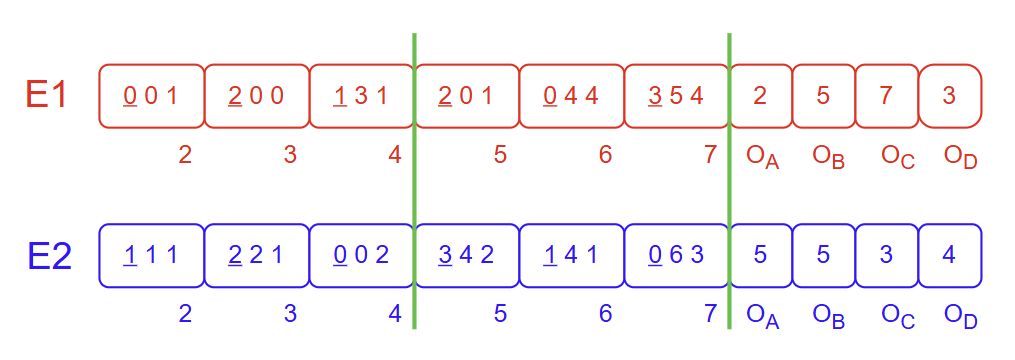
\includegraphics[scale = 0.55]{Bilder/BeispielTwoPointCrossover.png}
    	\caption{Eltern-Chromosomen Two-Point Rekombination}
    	\label{fig:twoPointCrossoverEltern}
    \end{subfigure}
    
    \hfill
    
    \begin{subfigure}[b]{\textwidth}
    	\centering
    	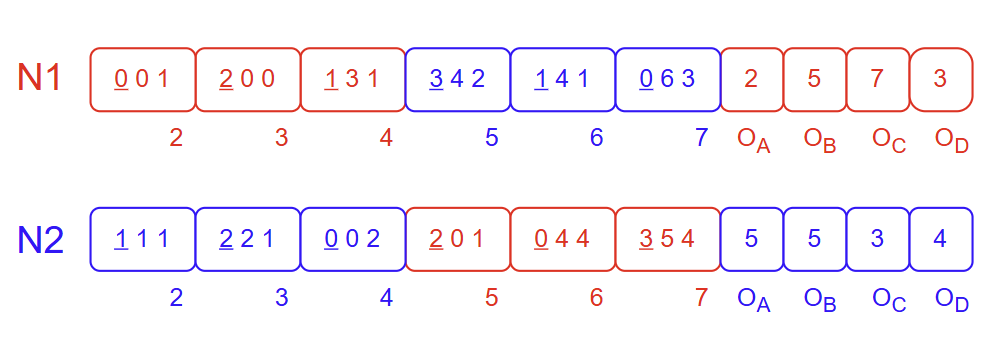
\includegraphics[scale = 0.55]{Bilder/BeispielTwoPointCrossover2.png}
    	\caption{Nachwuchs-Chromosomen Two-Point Rekombination}
    	\label{fig:twoPointCrossoverNachwuchs}
    \end{subfigure}
    \caption{Two-Point Rekombination, angelehnt an \cite{torabi_using_2022}}
    \label{fig:twoPointGesamt}
\end{figure}

Zu beobachten ist, dass die Eltern-Chromosomen an jeweils zwei Stellen aufgeteilt werden (grün).
Die Nachwuchs-Chromosomen bilden sich anschließend abwechselnd aus den Teilstücken der beiden Eltern-Chromosomen.
In der Abbildung \ref{fig:twoPointGesamt} wird dieser Prozess deutlich, indem die Chromosomenteile des ersten Elternteils rot und des zweiten blau markiert sind.


\subsection{Uniform Rekombination}
\label{subsubsec:unformCrossover}
Die Erläuterung der \emph{Uniform Rekombination} basiert auf \cite{syswerda_uniform_1989}.\\
Der größte Unterschied zwischen Uniform Rekombination und One-Point / Two-Point Rekombination ist die Verwendung einer Maske. 
Die Maske ist genauso lang wie die Eltern-Chromosomen selbst und beinhaltet für jede Stelle binäre Werte.
Diese Werte geben jeweils an, von welchem Elternteil die jeweilige Stelle im Chromosom des Nachwuchses stammen soll.
Der zweite gebildete Nachwuchs bekommt in diesem Prozess das Gen des jeweils anderen Elternteils.\\
Anhand der Abbildung \ref{fig:uniformGesamt} lässt sich die Uniform Rekombination beispielhaft erklären:

\begin{figure}[H]
    \centering
    \begin{subfigure}[b]{\textwidth}
    	\centering
    	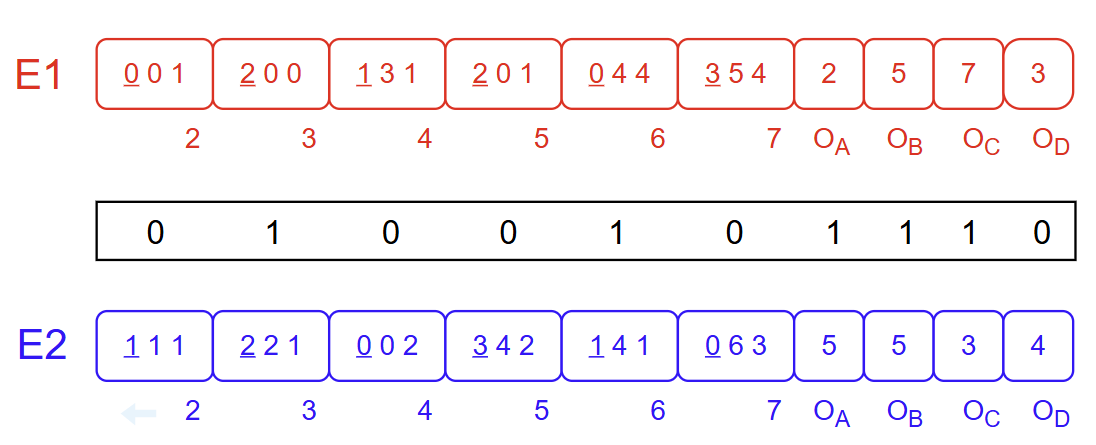
\includegraphics[scale = 0.755]{Bilder/BeispielUniformCrossover.png}
    	\caption{Eltern-Chromosomen Uniform Rekombination}
    	\label{fig:uniformCrossoverEltern}
    \end{subfigure}
    
    \hfill
    
    \begin{subfigure}[b]{\textwidth}
    	\centering
    	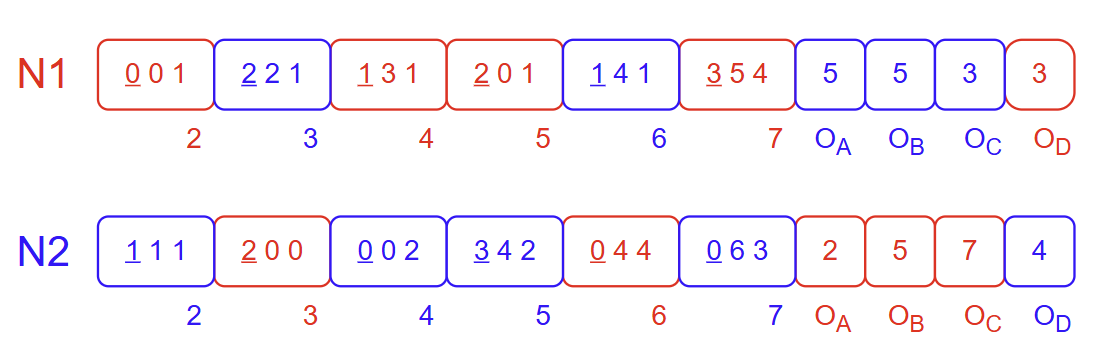
\includegraphics[scale = 0.49]{Bilder/BeispielUniformCrossover2.png}
    	\caption{Nachwuchs-Chromosomen Uniform Rekombination}
    	\label{fig:uniformCrossoverNachwuchs}
    \end{subfigure}
    \caption{Uniform Rekombination, angelehnt an \cite{torabi_using_2022}}
    \label{fig:uniformGesamt}
\end{figure}

Abbildung \ref{fig:uniformCrossoverEltern} zeigt die Ausgangssituation mit den beiden Eltern-Chromosomen (E1 und E2) in rot und blau.
Zwischen den beiden Eltern-Chromosomen wird schwarz die Maske angezeigt.
Diese wird zufällig binär gefüllt, bis sie die Länge der beiden Eltern-Chromosomen erreicht.\\
Im folgenden Schritt werden die Nachwuchs-Chromosomen unter Anbetracht der Maske erzeugt.
Der entsprechende Index des Knotens kann jeweils unterhalb der Eltern-Chromosomen abgelesen werden.
Für den ersten Wert der Maske ergibt das den Knotenindex 2.
In diesem Beispiel enthält der erste Wert der Maske eine 0.
Dementsprechend wird für den Knoten mit dem Index 2 des ersten Nachwuchs-Chromosoms (N1) der jeweilige Knoten des ersten Eltern-Chromosoms (E1, rot) verwendet.
Das zweite Nachwuchs-Chromosom (N2) bekommt demnach den entsprechenden Knoten aus dem zweiten Eltern-Chromosom (E2, blau).\\
Für den darauffolgenden Index hat die Maske den Wert 1.
Dies bedeutet, dass die Vererbungen andersherum ablaufen: N1 bekommt den Knoten von E2 und N2 bekommt den Knoten von E1.
Dieser Prozess wird für alle Indices ausgeführt.
Die Abbildung \ref{fig:uniformCrossoverNachwuchs} zeigt die resultierenden Ergebnisse für dieses Beispiel der Uniform Rekombination.


\subsection{Rekombinationsraten}
\label{subsec:rekombinationsraten}

In den letzten Abschnitten wurden unterschiedliche Rekombinationsalgorithmen erläutert.
Der Rekombinationsschritt wird allerdings nicht für jedes Nachwuchs-Chromosom verwendet.
Dieser wird nur zu einer bestimmten Wahrscheinlichkeit ausgeführt, welche mit der \emph{Rekombinationsrate} beschrieben wird.
Die Effektivität des (C)GP-Systems hängt unter anderem von der richtigen Wahl der Rekombinationsrate ab. \cite{hassanat_choosing_2019}\\
Um das bestmögliche (C)GP-System zu erhalten, sollte das richtige Verhältnis aus \emph{Exploration} (dt. Erforschung) und \emph{Exploitation} (dt. Ausbeutung) des Lösungsraums erzielt werden. 
Exploration ist dabei der Prozess, neue Bereiche des Lösungsraums zu erkunden, während bei der Exploitation bereits erkundete Regionen des Lösungsraums näher betrachtet werden.
Eine Stellschraube, um den eigenen Prozess dahingehend zu steuern, ist die Rekombinationsrate. \cite{crepinsek_exploration_2013}
Wird die Rekombinationsrate sehr hoch eingestellt, wird zu einem hohen Maß Exploration betrieben. 
Dies führt allerdings dazu, dass die Exploitation niedrig gehalten wird und somit die optimalen Lösungen verfehlt werden. \cite{pavai_survey_2017}\\
In unterschiedlichen Papern werden verschiedene Herangehensweisen vorgeschlagen, diesen Parameter zu wählen.
Teilweise widersprechen sich diese Aussagen.
Ziel dieser Arbeit ist es, unter anderem einen Einblick zu bekommen, wie man die Rekombinationsrate richtig wählen kann und welche Auswirkungen sie auf die Güte von CGP-Lösungen hat.

Die folgenden Abschnitte geben einen Einblick über die unterschiedlichen Möglichkeiten, die Rekombinationsrate zu setzen.

\subsubsection{Konstante Rekombinationsrate}
\label{subsubsec:konstanteCrossover}

Wie von Hassanat et al. beschrieben, ist die konstante (statische) Rekombinationsrate die übliche Form. 
Als geläufiges Beispiel wird in ihrem Paper der Wert 0,9 für die Rekombinationsrate vergeben. \cite{hassanat_choosing_2019} 
Dies bedeutet, dass zur Initialisierung des CGP ein fester Wert für die Rekombinationsrate gewählt wird.
Dieser gilt für alle Generationen gleichermaßen und wird nicht verändert.\\
Diese \glqq klassische\grqq\space Form der Rekombination kann in der Evaluation der praktischen Tests dazu verwendet werden, um die erste Forschungsfrage zu beantworten.
Durch diese einfachste Form der Rekombinationsrate kann überprüft werden, ob CGPs ohne oder mit (klassischer) Rekombination effizienter sind.\\
Mit Hilfe der in den nächsten Abschnitten beschriebenen Anpassungen der Rekombinationsrate kann anschließend überprüft werden, ob die Effizienz von CGP mit Rekombination weiter verbessert werden kann.

\subsubsection{Linear fallende Rekombinationsrate}
\label{subsubsec:CleggCrossover}

Clegg et al. präsentieren in ihrem Paper aus 2007 eine neue Form der Rekombination.
Dabei treffen sie auch einige Aussagen über die Rekombinationsrate, die in diesem Abschnitt näher betrachtet werden sollen. \cite{clegg_new_2007}\\
Sie beobachten, dass sich für höhere Rekombinationsraten eine schnellere Konvergenz der Fitness innerhalb der ersten Generationen einstellt.
Gleichzeitig stellen sie fest, dass in ihrem Beispiel ab der 200. Generation Rekombination keinen signifikanten Vorteil in der Performance liefert.\\
Aus diesen beiden Beobachtungen konstruieren sie eine neue, dynamische Rekombinationsrate.
Diese beginnt bei einem hohen Startwert von 0,9 und sinkt linear, bis eine Rekombinationsrate von 0,0 erreicht wird. 
In ihrem Beispiel legen die Autoren über händische Analysen eine Generation fest, bis zu welcher die Rekombinationsrate auf 0,0 fallen soll.\\
Innerhalb des praktischen Teils dieser Arbeit wird 0,9 für den Startwert der Rekombinationsrate übernommen, um die Anzahl der Parameter in der Hyperparameteranalyse zu reduzieren.
Ebenfalls ist es ein Vorteil, nur einen variablen Parameter pro Rekombinationsraten-Typ zu verwenden, da gegebenenfalls die Änderungen innerhalb der Ergebnisse für die verschiedenen Parameter besser miteinander verglichen werden können.\\
Der einzige variable Parameter für die linear fallende Rekombinationsrate ist in dieser Arbeit die Rate, die nach jeder Generation von der alten Rekombinationsrate abgezogen werden soll, um die neue Rekombinationsrate zu erhalten.

\subsubsection{One-Fifth-Regel angewandt auf die Rekombinationsrate}
\label{subsubsec:oneFifthCrossover}

Die \emph{One-Fifth-Regel} gibt es bereits für andere Parameter von GP, wie beispielsweise für die \emph{Mutationsrate}, die in Abschnitt \ref{subsec:Mutation} näher erläutert wird.
Diese Regel wird ebenfalls im Paper von Milano und Nolfi verwendet.
Dabei handelt es sich um einen Weg, die Mutationsrate automatisch und dynamisch an die Problemcharakteristiken und die evolutionäre Phase anzupassen. \cite{milano_scaling_2018}\\
Betrachtet wird bei dieser Regel das Fitness-Verhältnis der Elitisten und der neuen Chromosomen.
In anderen Worten werden die Kinder mit ihren Eltern verglichen.
Erzielt werden soll ein Verhältnis von 20\%.
Das heißt, dass 20\% der Nachwuchs-Chromosomen eine bessere Fitness aufweisen sollen als ihre Eltern.
Wird dieses Verhältnis unter- oder übertroffen, wird der jeweilige Parameter verkleinert oder vergrößert. \cite{doerr_self-adjusting_2019}

In dieser Arbeit soll die One-Fifth-Regel für die dynamische Anpassung der Rekombinationsrate herangezogen werden.
Um nur den Rekombinationsschritt zu bewerten und nicht den Mutationsschritt, muss die Bewertung der Fitness vor der Mutation geschehen.
Dementsprechend wird für die One-Fifth-Regel in dieser Arbeit direkt nach dem Rekombinationsschritt die Fitness der Eltern- mit der Fitness der Nachwuchs-Chromosomen verglichen.
Anschließend wird betrachtet, ob 20\% der Kinder eine bessere Fitness aufweisen als ihre Eltern.
Wird dieser Wert übertroffen, wird die Rekombinationsrate mit 1,1 multipliziert, um den Erfolg des Rekombinationsschritts auszuschöpfen.
Andernfalls wird die Rekombinationsrate mit 0,9 multipliziert und somit verringert.


\subsubsection{Rekombinationsrate mit Offset}
\label{subsubsec:offsetCrossover}
Torabi et el. beschreiben in ihrem Paper eine neue Rekombinationsstrategie \cite{torabi_using_2022}.
Dabei verwenden sie einen Hyperparameter, der den \emph{Offset der Rekombination} definieren soll.
Das heißt, dass die Rekombination in ihrer Strategie in den ersten Generationen nicht angewendet wird, sondern erst zu einer bestimmten Generation beginnt.
Wie dieser Hyperparameter bestimmt wurde und welche Größenordnung dieser einhalten sollte, wird in dem Paper allerdings nicht erwähnt.

Torabi et al. behaupten außerdem, dass ihre Strategie \glqq den richtigen Kompromiss aus Exploration und Exploitation\grqq\space erreiche. \cite{torabi_using_2022}
Vergleicht man diese Behauptung mit der Aussage von Clegg et al., stellt man fest, dass sich diese Thesen widersprechen.
Während Clegg et al. vor allem in den ersten Generationen auf Rekombination setzen, da der Rekombinationsschritt hier zu einer höheren Fitness-Konvergenz führen soll, meiden Torabi et al. in ihrer Strategie Rekombinationen in den ersten Generationen völlig. \cite{clegg_new_2007}\\
Ein Ziel dieser Arbeit ist es herauszufinden, ob sich ein Offset in der Rekombination als sinnvoll erweist oder ob sich dieser nur für die Rekombinationsstrategie eignet, die Torabi et al. in ihrem Paper eingeführt haben.


\section{Evolutionärer Operator: Mutation}
\label{subsec:Mutation}

Der zweite evolutionäre Operator ist die Mutation.
Sie wird nach der Rekombination ausgeführt.
Anders als bei der Rekombination werden bei der Mutation nicht zwei, sondern nur ein Chromosom einbezogen und daraus ein neues Chromosom erstellt.
In diesem Prozess werden Teile des Genotyps des Chromosoms zufällig verändert, um daraus einen neuen Genotyp zu erzeugen. \cite{milad_taleby_ahvanooey_survey_2019}\\
Für \emph{probabilistische Mutation} wird eine Mutationsrate verwendet, um die Wahrscheinlichkeit anzugeben, mit der ein Gen mutiert wird.
Dadurch kann es allerdings dazu kommen, dass das Chromosom vor und nach der Mutation zwar unterschiedliche Genotypen aufweist, sich die aktiven Knoten allerdings nicht voneinander unterscheiden.
Dies hat zur Folge, dass sich der Lösungsansatz des CGPs bezüglich des Ausgangsproblems nicht ändert, obwohl bereits eine Mutation ausgeführt wurde.
Die Fitness des CGPs kann sich in so einem Fall nicht verbessern.
Um dieses Problem in den Griff zu bekommen, wird in dieser Arbeit die \emph{Single (Active) Mutation} herangezogen.
In diesem Algorithmus werden zufällige Gene eines Chromosoms verändert, bis ein aktiver Knoten mutiert wurde.
Anschließend bricht der Mutationsalgorithmus ab. \cite{miller_cartesian_2020}
Dies hat zusätzlich den Vorteil, dass keine Mutationsrate angepasst werden muss, was die Hyperparameteranalyse weniger rechenintensiv macht.

Die Veränderung eines Gens innerhalb der Mutation wird vorgenommen, indem das ausgewählte Zeichen des Genotyps zufällig geändert wird \cite{koza_survey_1995}. 
Dies hat für unterschiedliche Knotenarten des entsprechenden Phänotyps verschiedene Effekte.\\
Ein Ausgangsknoten hat als relevanten Parameter nur seinen Vorgängerknoten.
Wird also ein Ausgangsknoten mutiert, wird die eingehende Kante zufällig neu belegt.
Dabei muss wie bei der Initialisierung beachtet werden, dass die Struktur von CGP erhalten bleibt.
In dieser Arbeit werden dementsprechend nur Vorgängerknoten gewählt, deren Index kleiner ist als der mutierte Knoten.\\
Anders als die Ausgangsknoten wird ein Rechenknoten durch mindestens zwei Parameter bestimmt: ein Rechenoperator und mindestens eine Eingangskante.
Welcher dieser Parameter mutiert werden soll, ist ebenfalls Zufall.
Wird eine Kante verändert, gelten die gleichen Regeln wie beim Mutieren eines Ausgangsknotens.
Wird der Rechenoperator mutiert, wird dieser zufällig neu aus den kodierten Rechenfunktionen gewählt.\\
Da ein Eingangsknoten nur aus den Dateneingängen besteht und keine Parameter enthält, können diese nicht mutiert werden und werden im Mutationsschritt nicht betrachtet.

Um die Single Active Mutation anhand eines Beispiels näher zu erläutern wird folgender Gentyp eines Chromosoms aus Abbildung \ref{fig:genotypNeu} erneut eingeführt.
Es wird angenommen, dass dieses Chromosom durch vorherige Rekombination entstanden ist und somit im nächsten Schritt mutiert werden soll.
Die folgende Abbildung \ref{fig:mutationGesamt} zeigt dieses Mutationsbeispiel:

\begin{figure}[H]
	\centering
	\begin{subfigure}[b]{\textwidth}
		\centering
		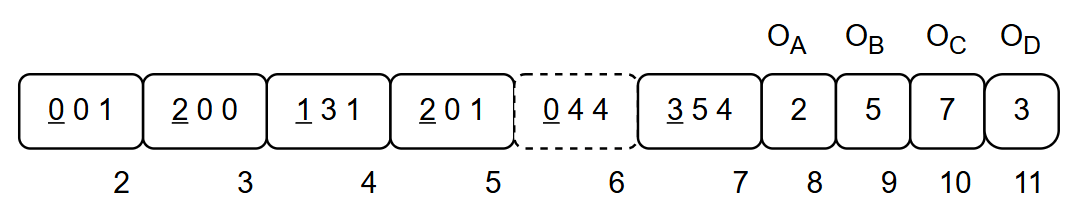
\includegraphics[scale = 0.55]{Bilder/TorabiBeispielGenotypNeu.png}
		\caption{Genotyp vor Mutation}
		\label{fig:genotypVorMutation}
	\end{subfigure}
	
	\hfill
	
	\begin{subfigure}[b]{\textwidth}
		\centering
		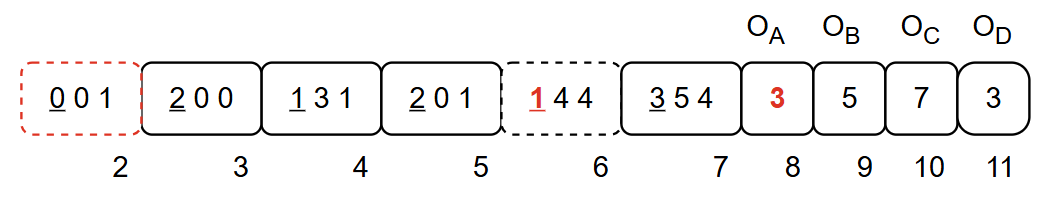
\includegraphics[scale = 0.568]{Bilder/GenotypNachMutation.png}
		\caption{Genotyp nach Mutation}
		\label{fig:genotypNachMutation}
	\end{subfigure}
	\caption{Single Active Mutation, angelehnt an \cite{torabi_using_2022}}
	\label{fig:mutationGesamt}
\end{figure}

Zu Beginn des Algorithmus wird ein zufälliger Index für die Mutation ausgewählt.
Angenommen dieser Index hat den Wert 6.
Dabei handelt es sich um einen Rechenknoten.
Da in diesem Beispiel die Rechenknoten jeweils 3 Parameter aufweisen, wird zufällig einer der drei Parameter für die Mutation bestimmt.
In diesem Beispiel wird der erste Parameter verändert, also der Rechenoperator.
Wie bereits in Tabelle \ref{table:kodierung} aufgezeigt, werden die Rechenoperationen durch 0 bis 3 kodiert.
Sei beispielsweise die zufällig gewählte Zahl für den Rechenoperator gleich 1.
Da der in diesem Schritt mutierte Knoten inaktiv ist, muss nach der Single Active Mutation erneut mutiert werden.\\
Angenommen der zufällig gewählte Index ist 8, was dem Index von $O_A$ entspricht.
Da es sich, um einen Ausgangsknoten handelt, muss ein neuer Vorgängerknoten zufällig gewählt werden.
Beispielsweise wird nun dieser Parameter mit dem Index 3 belegt.
Da dieser Knoten Teil der aktiven Knoten ist, terminiert hier der Mutationsalgorithmus.
Die Abbildung \ref{fig:genotypNachMutation} zeigt das Ergebnis des Mutationsbeispiels (mit Kennzeichnung der neuen aktiven / inaktiven Knoten).
Die mutierten Teile des Chromosoms, sowie der neu entstandene inaktive Knoten werden rot hervorgehoben.


\section{Evaluation Fitness, Stopp-Kriterium und Ergebnis}
\label{sec:fitness,StopKrit,Ergebnis}

Nachdem der Mutationsschritt für alle Chromosome der Population ausgeführt wurde, findet erneut ein Evaluationsschritt statt.
Dabei wird für jedes Chromosom ein Fitness-Wert bestimmt, der bewertet wie exakt die Trainingsdaten durch das Chromosom beschrieben werden. \cite{milad_taleby_ahvanooey_survey_2019}
Die Berechnung der Fitness hängt wie in Abschnitt \ref{sec:evalUndSelektion} erläutert von dem zu lösenden Ausgangsproblem ab.\\
Sobald für alle Chromosome einer Population ein Fitness-Wert bestimmt wurde, werden diese auf das \emph{Stopp-Kriterium} geprüft.
Dieses gibt an, ab welcher Bedingung ein Algorithmus als konvergiert gilt.
Im Beispiel von Cui et al. ist diese Bedingung bei symbolischen Regressionsbenchmarks für $Fitness < 0,01$ erfüllt. \cite{affenzeller_positional_2024}\\
Wird das Stopp-Kriterium erfüllt, wird der CGP-Algorithmus abgebrochen.
Das Ergebnis ist das beste Chromosom der letzten Generation.
Dieses löst das Ausgangsproblem hinreichend gut.
Andernfalls wird eine weitere Iteration des CGP-Algorithmus gestartet. 
Dabei werden erneut Selektion, Rekombination und Mutation ausgeführt, um eine bessere Lösung des Ausgangsproblems zu finden.

\section{Bayes'sche Analyse}
\label{sec:bayesian}

Für die Evaluation der Ergebnisse werden in diesem Abschnitt statistische Grundlagen zur \emph{Bayes'schen Analyse} erläutert.\\
Der Satz von Bayes (Bayes'sches Therorem) bietet Grundlagen zur Berechnung der bedingten Wahrscheinlichkeit.
Zu Beginn wird eine Anfangshypothese über das Ergebnis eines Wahrscheinlichkeitsproblems angenommen.
Mit zusätzlichen Informationen wird die Anfangshypothese schließlich korrigiert.
Das Ergebnis ist eine neue Wahrscheinlichkeit, die alle vorhandenen Informationen einschließt. \cite{peyrolon_definition_2020}

Vereinfacht dargestellt funktioniert die Anwendung des Satzes von Bayes in der Bayes'schen Analyse wie in folgender Abbildung \ref{fig:bayesianInference}.

\begin{figure}[H]
	\centering
	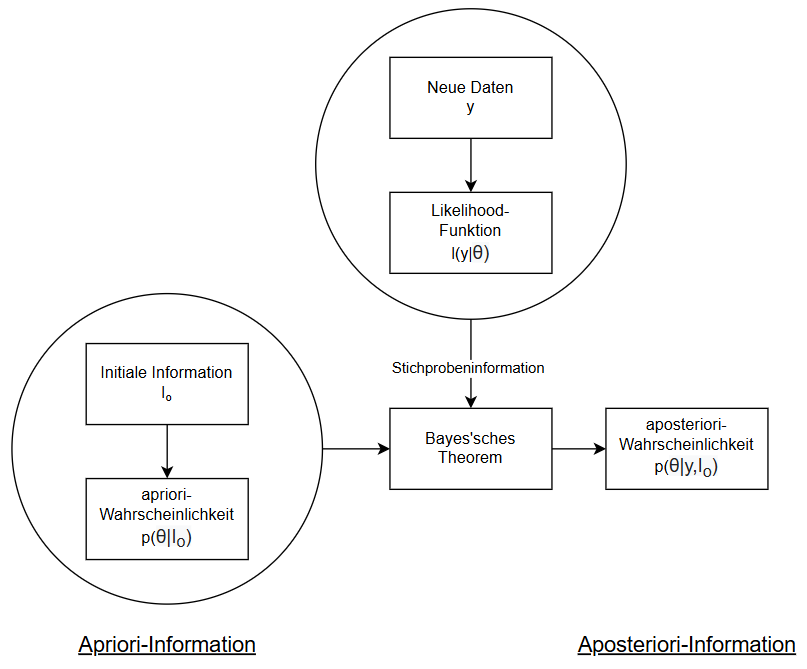
\includegraphics[scale = 0.8]{Bilder/bayesianInterence.png}
	\caption{Bayes'sche Analyse, angelehnt an \cite{nenning_bayessche_1980}}
	\label{fig:bayesianInference}
\end{figure}

Zu Beginn wird die Realität als Modell mit bestimmten Annahmen ($\theta$) vereinfacht.
Diese ursprünglichen Annahmen werden als Wahrscheinlichkeitsverteilung (\emph{apriori-Wahr\-schein\-lich\-keit}) dargestellt. 
Aus den neuen Daten y kann die sogenannte
\emph{Likelihood-Funktion} errechnet werden, die eine Dichtefunktion für die Beobachtung y darstellt unter der Bedingung, dass $\theta$ zutrifft.
Mit Hilfe des Bayes'schen Theorems können die apriori-Dichtefunktion und die Stichprobeninformationen miteinander verknüpft werden.
Das Ergebnis ist eine neue Wahrscheinlichkeitsverteilung für $\theta$ (\emph{aposteriori-Wahrscheinlichkeit}). \cite{nenning_bayessche_1980}
Mit diesem Vorgehen kann also mit Hilfe von empirischen Daten eine Wahrscheinlichkeitsverteilung für ein Modell gefittet werden.

In dieser Arbeit werden basierend auf \cite{cui_equidistant_2023} zwei Modelle verwendet: das \emph{Plackett-Luce-Modell} und das \emph{Gammaverteilung-basierte Modell}.\\
Mit Hilfe des Plackett-Luce-Modells können die Wahrscheinlichkeiten berechnet werden, mit denen die jeweiligen CGP-Konfigurationen besser als alle anderen Konfigurationen sind.
Demnach kann eine Reihenfolge bestimmt werden, die die Effizienz der Konfigurationen sortiert angibt.
Das verwendete Modell basiert auf dem Plackett-Luce-Modell, das von Calvo et al. eingeführt wird. \cite{cui_equidistant_2023, calvo_plackett_luce}\\
Für die Auswertung mit Hilfe des Gammaverteilung-basierten Modells wird der Code von Pätzel verwendet (\cite{patzel_dpaetzelcmpbayes_2024}). 
Dieser ermöglicht es nicht-negative Daten zu vergleichen und daraus die Wahrscheinlichkeitsverteilung von $\mu_{config}$ zu schätzen.
$\mu_{config}$ ist dabei eine zufällige Variable, die dem jeweiligen Mittelwert der Iterationenzahl entspricht, die gebraucht werden, um eine CGP-Lösung konvergieren zu lassen.
Für jede CPG-Konfiguration kann so ein 95\% HPDI (\emph{highest posterior density interval}) von $\mu_{config}$ bestimmt werden.
Dies bedeutet, dass innerhalb dieses Intervalls 95\% der Ergebnisse liegen. \cite{cui_equidistant_2023}
Dadurch können die Streuungen der Iterationszahlen für jede CGP-Konfiguration miteinander verglichen werden, ohne von einer gleichverteilten Dichtefunktion ausgehen zu müssen.

Pätzel verwendet in seinem Code das \emph{Markov Chain Monte-Carlo (MCMC) Sampling} zur Berechnung der Verteilungen \cite{patzel_dpaetzelcmpbayes_2024, cui_equidistant_2023}.
Bei MCMC werden mehrere Tausend Kombinationen von Parameterwerten ($\mu_1$, $\sigma_1$, $\mu_2$, $\sigma_2$, v) generiert, die jeweils zwei verschiedene Gamma-Wahrscheinlichkeitsverteilungen darstellen.
Jede Wertekombination ist repräsentativ für glaubwürdige Parameterwerte, die gleichzeitig die eingehenden Daten und die vorherigen Verteilungen berücksichtigen.
Diese Parameterwerte werden anschließend zusammengefasst. \cite{kruschke_bayesian_estimation}

